\section{Implementation}

\sys{} consists of multiple data processing, code rewriting, and content delivery steps, making up a full debloating pipeline. 
Initially, our data-analysis step processes the code-coverage traces from web application users and performs the clustering based on the usage data and feature usage. 
Our system incorporates clustering metrics to determine the optimal number of clusters based on code-coverage information, but system operators can decide to modify this configuration based on other post-debloating factors such as LLOC reduction. 

\subsection{Processing the code-coverage information}

For all users of each web application, we extract the list of file and line coverage information. 
Our next task is to identify clusters of code-coverage data based on application usage similarity. 
In order to cluster similar profiles together, we train an unsupervised clustering model based on file names and file paths. 
This decision is based on the intuition that the architecture of popular web applications provides an organic hierarchy of their underlying modules. 

\subsubsection{Vectorizing covered file paths} 
Previously, we argued that file paths and file names are accurate indicators of the underlying feature in the web application based on user interactions and code-coverage traces. 
Based on this observation, we vectorize covered file paths and use TF-IDF algorithm to extract important terms from our corpus of data. 
Throughout this process, we experimentally identified that ignoring common terms that appeared in more than 50\% of the file paths (e.g., \texttt{vendor}, \texttt{wp-admin}, etc.) will yield the best results. 


\subsubsection{Clustering code-coverage information} We use the features returned by the TF-IDF processing in combination with K-Means clustering. 
On one end, we build a single cluster which acts as the baseline for our debloating measurements. 
This cluster which contains the code-coverage of all users resembles the debloating structure of Less is More by Amin Azad et al.~\cite{lessismore}. 
On the other end, we can assign a unique cluster for each user. 
By doing so, each user receives their own uniquely debloated web application which ensures the maximum tailoring of features. 
We argue that the optimal number of clusters lies in between the two extremes, such that the debloating metrics (e.g., code, CVE, and sensitive function call reduction) are optimized while keeping the number of clusters manageable. 

Moreover, as we demonstrate later in Section~\ref{sec:augmented_coverage}, it is beneficial to group users with similar behavior in the same cluster as they will augment each others' code-coverage. 
This aggregation reduces the likelihood of users running into removed features (i.e., features that they did not exercise during the training of the system which were subsequently removed) as other users with similar usage patterns may have already covered the code responsible for the desired feature. 

Web applications sometimes create temporary PHP files for caching purposes. 
Other interactions with the web applications such as installing a new module can also result in the introduction of new PHP code. 
For our debloating scheme, we consider an application at a stable state (i.e., required plugins and modules are already installed prior to debloating). 
Therefore, we perform a clean up step through which we remove references from code-coverage traces that point to non-existing files in the original version of the applications. 

Our goal in this paper is to demonstrate the debloating performance of popular web applications in their original format. 
Specific to our user study, our clean up step will essentially remove newly installed modules during the user study experiments, but will keep the code in the original application that enables users to install new modules. 

\begin{figure}[]
    \centering
    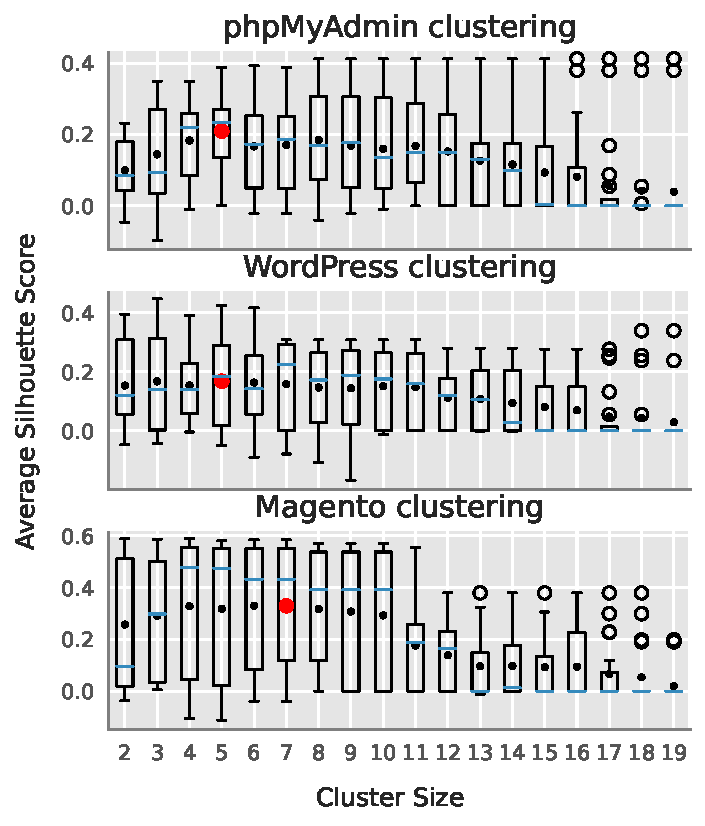
\includegraphics[width=0.50\textwidth]{figures/dbltr/silhouette.pdf}
    \caption{Distribution of Silhouette scores of each cluster. The average score for each cluster is marked with a solid dot and the maximum average is marked with a solid red dot.}
    \label{fig:silhouette_scores}
    \vspace{-1em}
\end{figure}

\subsubsection{Determining the optimal number of clusters} 
\label{sec:num-clusters}

We can determine the optimal number of clusters based on a variety of source code similarity (i.e., file name and path) as well as debloating metrics (i.e., CVE reduction, and CAC reduction). 
\sys{} bases its decision on file similarity, concretely file name and path information that is readily available before clustering is performed. 

\sys{} then calculates the Silhouette score metric~\cite{kaufman2009finding} for the clusters. 
For each data point, the Silhouette score measures the similarity of the given data point to other points in its own cluster compared to points from other clusters. 
\sys{} determines the number of clusters by maximizing the average Silhouette score. 

Figure~\ref{fig:silhouette_scores} depicts the distribution of Silhouette scores based on the cluster size for each of the web applications in our dataset. 
The average score for each cluster size is shown by a solid dot, and optimal cluster size is depicted with a solid red dot. 
Given the ways that the 60 administrators used the evaluated web applications during our user study, the optimal number of clusters are as follows: 5 clusters for phpMyAdmin, 5 for WordPress, and 7 for Magento. 
For certain applications such as Magento, a range of values for the cluster size may be near optimal, in all cases, we selected the number that maximizes the average Silhouette scores.
As the number of clusters increase, we reach an optimal cluster size. 
Beyond this point, by approaching the extreme cluster size (e.g., 19 clusters), we produce many highly-similar small clusters, which reduces the average Silhouette score to close to zero. 

\subsubsection{Debloating the applications} For each cluster, we merge the code-coverage information for all the users of that cluster, and then use the aggregate file and line coverage information to identify unused files and functions and debloat them. 

The process of debloating consists of neutralizing unused files and functions by replacing them with a routine that blocks the further execution of the code. 
This step provides us with \emph{N} copies of the original application, with \emph{N} being the optimal number of clusters determined by \sys{}. 
Each debloated cluster caters to the use cases of its underlying users. 
Finally, we calculate the debloating metrics such as size, CVE, and CAC reduction for each cluster. 
We discuss these results in more detail in Section~\ref{sec:debloatingresults}.

\subsection{Content delivery}

The second stage of the \sys{} pipeline is responsible for serving the debloated web applications and seamlessly routing users to their underlying debloated web applications. 

\sys{} implements a reverse-proxy module based on OpenResty~\cite{openresty}, which is a popular high performance scalable web platform that extends NGINX and provides content manipulation APIs through Lua code. 
This is depicted in Figure~\ref{fig:system_architecture} as step 3. 

We implement the login-detection logic as a Lua module for OpenResty. 
This module is responsible for detecting successful login requests, extracting username and session cookie information, as well as storing and retrieving the user to debloated web application mappings from the data store. 
A high-level representation of the login detection module for phpMyAdmin is depicted in Listing~\ref{lst:lua}.

During the debloating stage, \sys{} produces mappings that directs our OpenResty module to redirect users to specific instances of debloated web applications. 
This information is stored in a Redis datastore along with active session-cookie-to-username mappings extracted by the Lua module. 

\definecolor{commentsColor}{rgb}{0.497495, 0.497587, 0.497464}
\begin{lstlisting}[caption=LUA configuration to detect successful logins and extract authentication cookies for phpMyAdmin,label=lst:lua,basicstyle=\footnotesize, float=tp, floatplacement=tbp, language={[5.0]Lua},commentstyle=\color{commentsColor}\textit, numbers=left, xleftmargin=5.0ex, breaklines=true]
-- phpMyAdmin Username extraction
if post_params ~= nil and (string.find(ngx.var.request_uri, "/") or string.find(ngx.var.request_uri, "index.php")) 
  then
    if post_params["pma_username"] ~= nil then
      username = post_params["pma_username"]
    end
end
-- phpMyAdmin Successful login detection
if ngx.var.request_method == "POST" and ngx.var.username ~= "" and ngx.status == 302 then
  -- Successful login detected extract session cookie
  for key, value in pairs(cookies) do
    if string.match(value:lower(), "phpmyadmin") then
      -- Store cookie value in Redis
\end{lstlisting}

For each web application, we provide a configuration file that defines the login endpoint, username form field, and the successful login indicator. 
In the example of phpMyAdmin, successful login is comprised of a POST request towards the login endpoint ``/'' or ``index.php'' that receives a 302 HTTP response code which redirects the user to the administration page of the application (Line 2 in Listing~\ref{lst:lua}). 

We extract the username from the POST request with the field name of ``pma\_username'' (Line 4) 
and then verify through the HTTP response code that we detected a successful login (Line 9). Finally, we extract the session cookie named ``phpmyadmin'' (Line 12) and store this user-to-session-cookie mapping in the Redis datastore for subsequent requests. 

For subsequent requests containing a valid session cookie, \sys{} first queries the username from the datastore and then determines the target web server based on the username mapping. 
Steps 4, 5, and 6 in Figure~\ref{fig:system_architecture} depict this process. 
Once the upstream web server is determined, traffic is routed to the corresponding web server. 
Any subsequent log-out requests and timeouts invalidate the session-cookie mapping.